\section{Introduction}
% 1,25 pp, including abstract and figure 1
%
Robotic systems are becoming more and more of a reality in orbital applications. Of interest here are those which may operate in On-Orbit Servicing and in Active Debris Removal missions [ETS-VII][Orbital Express][DEOS][Cinese mission][eDeorbit]. To tackle the related control challenges we present here an autonomy-based approach, in which the robot is commanded through a precomputed reference trajectory, corrected by a tracking controller, to account for intrinsic planning and execution errors. We focus on the task of grasping a defective, tumbling target satellite (from here on, the Target) by means of a free-floating robot, consisting of a non-actuated chaser satellite (from here on, the Chaser) carrying a kinematically redundant robot manipulator. These are shown in Fig.~\ref{fig:facility}.

The task of grasping a target satellite with a free-floating (CHECK) robot was already performed in space in [ETS-VII] and in [Orbital Express], however only for the case of a cooperative Target. When the Target cannot be attitude controlled and does not present visual or structural features to aid its grasping, then it is generally termed non-cooperative. In this case, the accomplishment of the robotic grasping task in autonomous mode presents some substantial challenges. The robot motion is dictated by that of the Target, which is generally unknown. The robot motion also has to be correctly synchronized with that of the Target, in order to meet and grasp some preselected grasping point on it, while satisfying motion constraints, such as workspace limits, kinematic and dynamic singularities, collision avoidance, as well as sensor-driven constraints, such as camera field-of-view boundaries and pixel velocity limits. Furthermore, due to the given free-floating dynamics in play, the effect of an impact during the contact phase can be very detrimental for accomplishing the task, since it can quickly bring the Target out of the range of the robot.

The grasping task of interest has been addressed extensively in the literature, first in the context of feedback control and then also in that of optimal control (see Section ???). While in the former the aim is to solve a regulation control problem, often taking advantage of the free-floating dynamics and redundancy of the Chaser, in the latter an open-loop approach is preferred, based on the idea of computing a feasible and optimal trajectory in real-time. Due to the highly constrained task, explained above, the use of a feasible trajectory is recognized to be of great importance.
\begin{figure}[t!]
\psfrag{x_1}[cc][cc][\FontFigBBB]{{\color{white}$\{\mathcal{I}\}$}}
\psfrag{t}[cc][cc][\FontFigBBB]{{\color{black}$\{\mathcal{T}\}$}}
\psfrag{g}[cc][cc][\FontFigBBB]{{\color{black}$\{\mathcal{G}\}$}}
\psfrag{e}[cc][cc][\FontFigBBB]{{\color{black}$\{\mathcal{E}\}$}}
\psfrag{b}[cc][cc][\FontFigBBB]{{\color{white}$\{\mathcal{B}\}$}}
\psfrag{q}[cc][cc][\FontFigBB]{{\color{black}$q$}}
\psfrag{r}[cc][cc][\FontFigBB]{{\color{black}$r$}}
\psfrag{g_pose}[cc][cc][\FontFigBB]{{\color{black}$\begin{bmatrix}\eta_t,~ \rho_t \end{bmatrix}$}}
\psfrag{camera}[cc][cc][\FontFigBB]{{\color{black}$\begin{bmatrix}\mu,~ r_c \end{bmatrix}$}}
\psfrag{c_pose}[cc][cc][\FontFigBB]{{\color{black}$\begin{bmatrix}\eta_c,~ \rho_c \end{bmatrix}$}}
\psfrag{t_pose}[cc][cc][\FontFigBB]{{\color{black}$\begin{bmatrix}q,~ r \end{bmatrix}$}}

\centering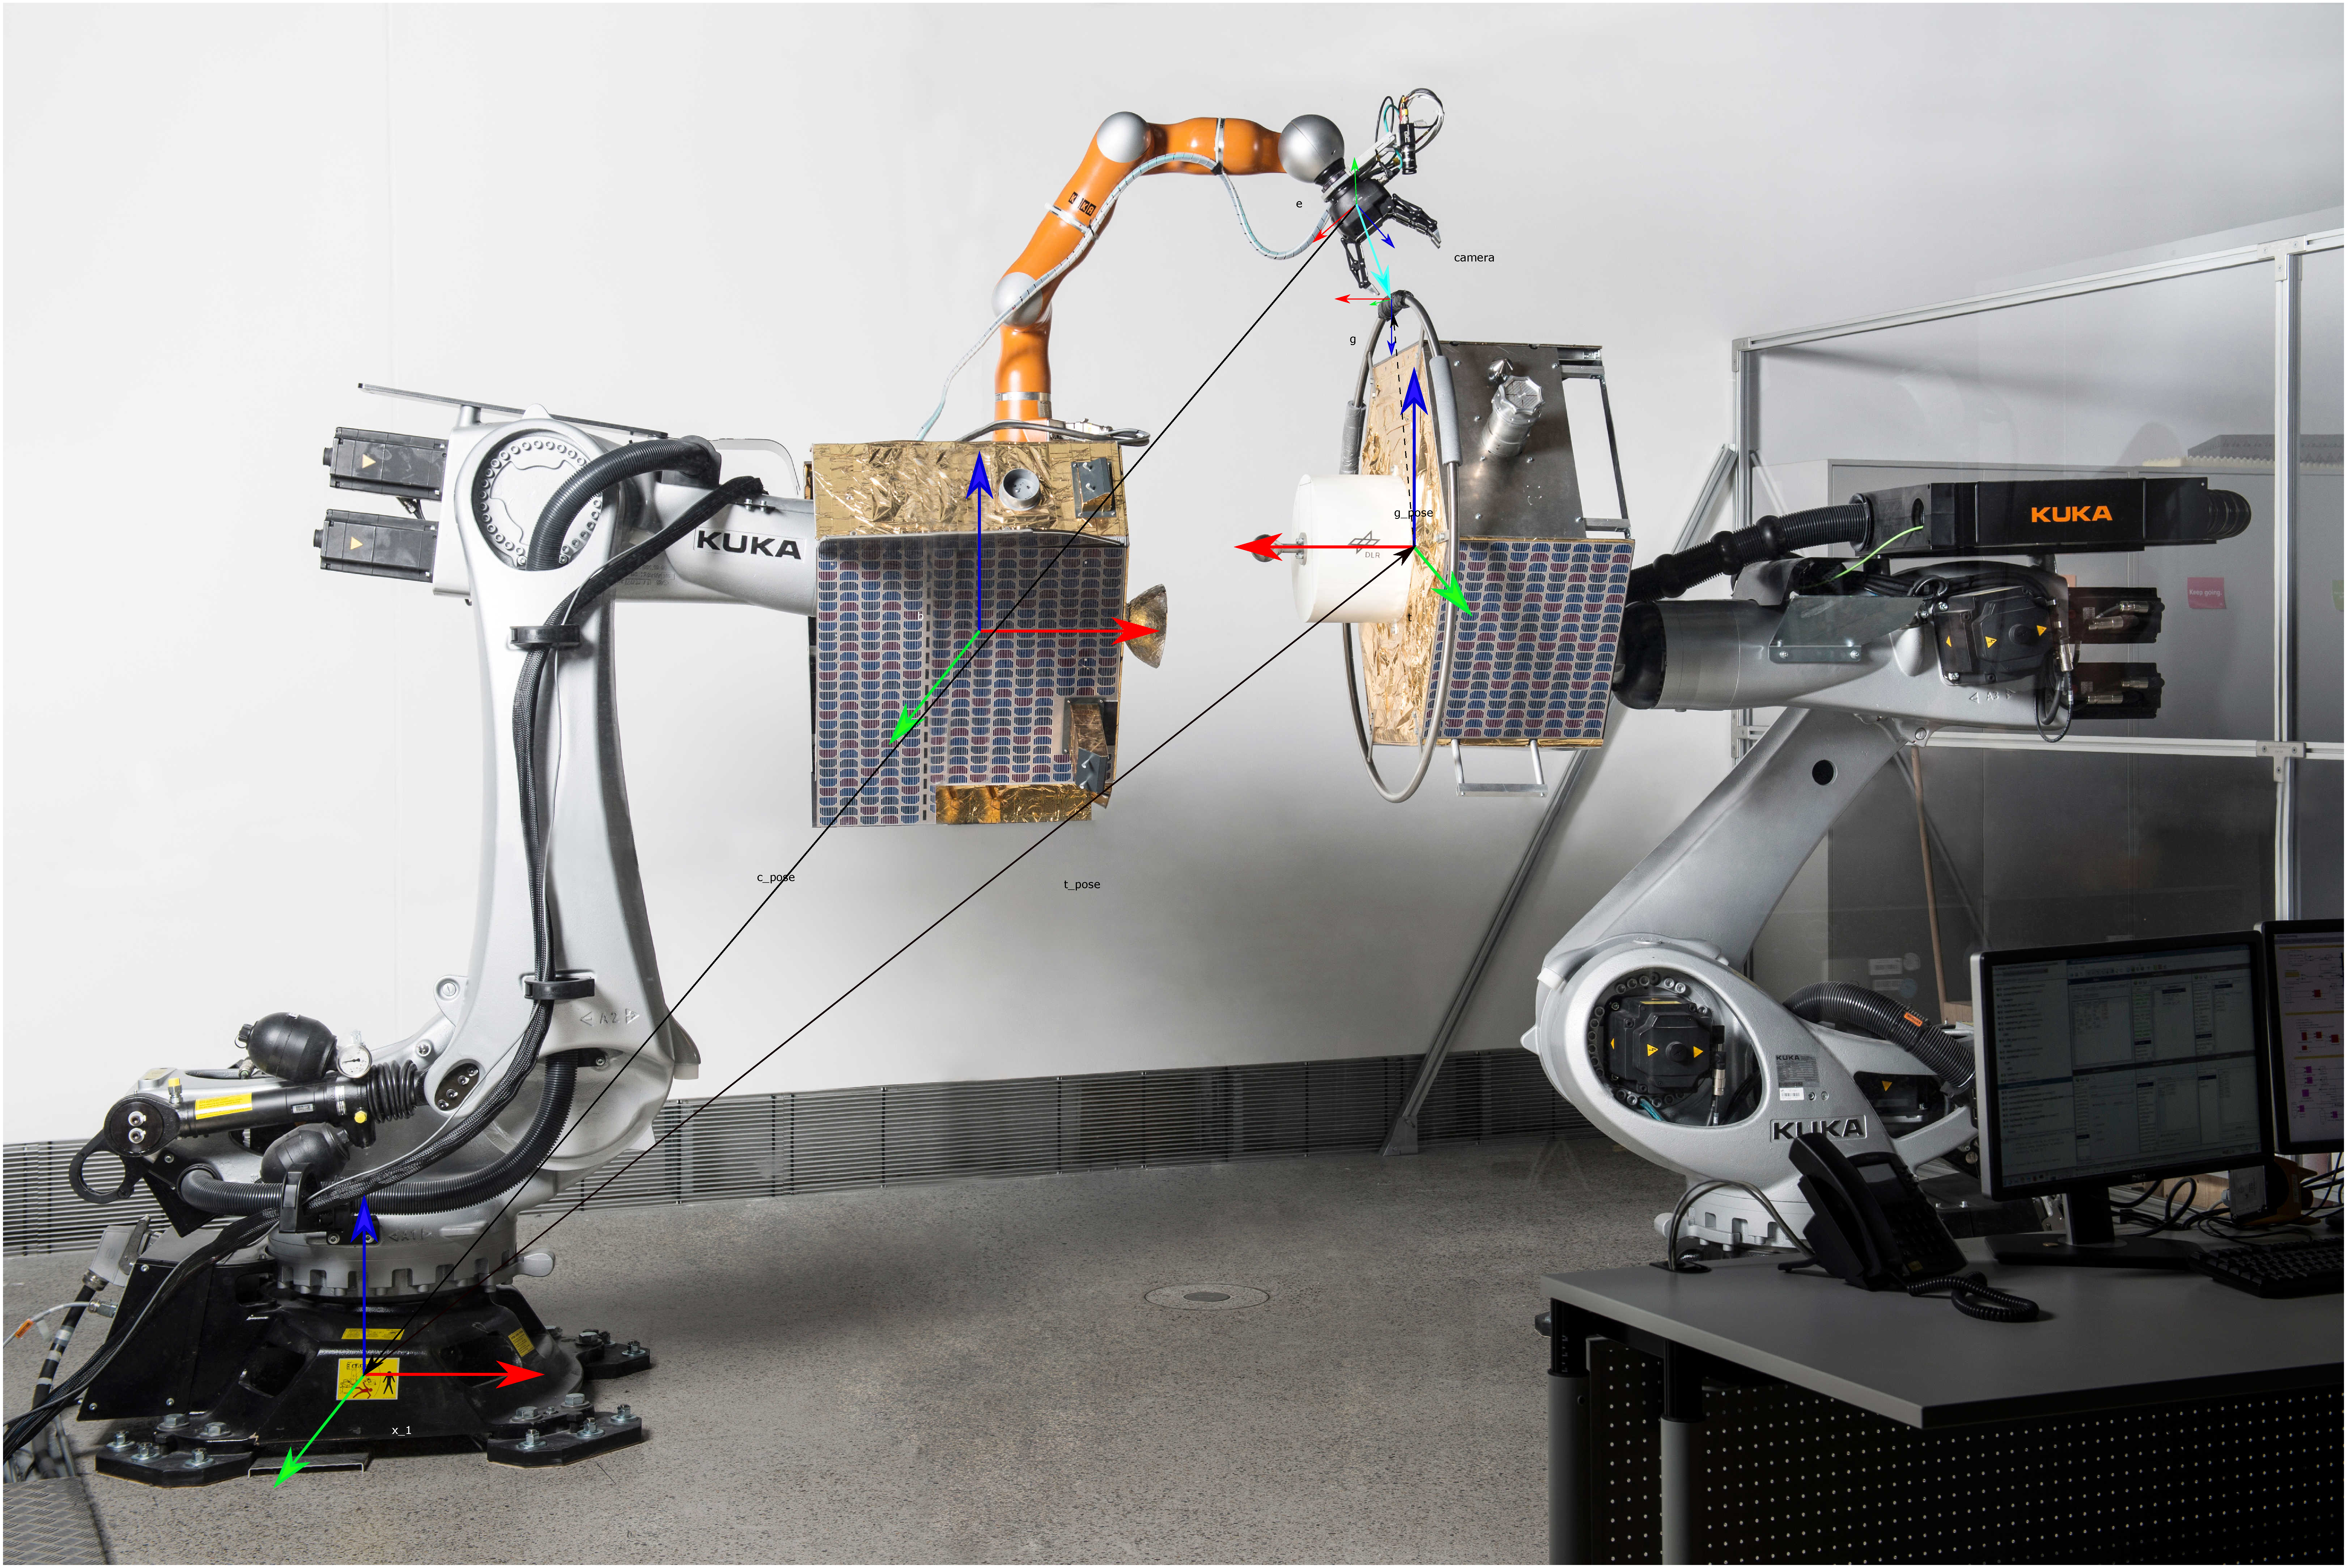
\includegraphics[angle=0,width=0.47\textwidth]{motiv.eps}
%\resizebox{0.48\textwidth}{!}{\fontsize{200}{200}\selectfont{\input{motiv.pdf_tex}}}
\caption{OOS-SIM experimental facility used to reproduce the gravity-free dynamics of the Chaser (left), carrying a Light-Weight Robot, and the Target (right). A camera is mounted on the gripper of the kinematically redundant manipulator, to allow visual servoing.}
\label{fig:facility}
%\vspace{-10pt}
\end{figure}

A gap in the methodology described above, which we want to close here, is that of having both the optimal control and the feedback control elements working together. A feedback controller alone does not provide any guarantee of convergence, given the presence of the constraints, let alone within a limited time window. At the same time, an open-loop approach is not robust to modelling errors and to contingencies, such as an impact. We present here a tracking controller for executing the grasping task of interest, which takes a reference trajectory from a database, generated off-line with a motion planner in simulation and feasible with respect to all relevant constraints, and superimposes on it sensor-based corrections to account for the discrepancy between the simulated and the real world.

The first phase of the task, the approach phase, is executed by means of a pose-based impedance visual servo, bringing the robot end-effector onto the grasping point on the tumbling Target. It is widely recognized that the robustness of a visual servo is significantly improved against modelling errors when performing tracking rather than regulation [Handbook 2016, Chapter 34, Visual Servoing]. The pose estimates are estimated throughout the motion with a Kalman filter, which is fed with the noisy pose estimates of a model-based visual tracking algorithm. The use of robot impedance control is intended to minimize the detrimental effect of an impact between the robot manipulator and the Target. In the following stabilization phase of the grasping task, in which the Target is already grasped but needs to be stabilized with respect to the Chaser, the reference trajectory provides a final configuration in which to let the system drift with decaying velocity, by virtue of the robot manipulator controller's damping action.

In this paper we present the tracking controller just described and its validation on DLR's OOS-SIM robotic facility, shown in Fig.~\ref{fig:facility}. This facility allows reproducing realistic orbital gravity-free dynamics in three-dimensions through hardware-in-the-loop simulation. The success of the controller requires a judicious interplay between the different elements involved: the motion planner, the pose-based impedance visual servo (including the Kalman filter and the visual tracking) and the free-floating robot impedance controller. Furthermore, the intrinsic uncertainty in the control problem at hand is handled with partial on-line replanning of the reference trajectory. Extensions of the functionality of the OOS-SIM facility to simulate the post-grasping tumbling motion of the satellite stack are also described.

The paper is then structures as follows. In the rest of this section, we present a relevant bibliography and a more detailed problem statement. In Section ??? we provide details of the applied methods, while in Section ??? we present the experimental results and their analysis. In Section ??? we provide our conclusions and views on future work.
%
\subsection{Related work - 0,5 pp}
%
Many approaches for grasping a free-tumbling Target mostly focus on feedback control methods [][][]%[Moosavian review paper][Papa's in IROS2013 check][Oda - Aghili's 22, 23, 24? Other?][ASTRA DeStefano]. 
and momentum control methods []%[Dimitrov][$IROS2006_Yoshida$]
. In [$Aghili_TRO2012$], the motion planning problem is solved for the approach phase of the grasping task. The planning is supported by a prediction of the Target's motion, achieved through an extended Kalman filter and noisy pose measurements of a laser camera system. The motion prediction occurs before any motion of the robot and the control strategy does not include a continuous visual feedback. An optimization problem is solved partly analytically and partly numerically, to minimize a penaltly cost, function of four weighted quantities: travel time, distance, line-of-sight angle of the laser camera and robot joint acceleration. The optimal control for the capturing maneuver is solved in the operational space of the robot manipulator and the robot manipulator kinematics and dynamics are as such not considered. Experiments are conducted on an experimental facility which reproduces the dynamics of the tumbling Target and of a robot manipulator end-effector with an attitude-controlled base. In []%[$Optimal_control_Robot_Detumbling_ICRA_2009.pdf$][$Optimal_time_Detumbling_JGND_2009.pdf$][$Aghili_ICRA2013$] 
a path planning method is presented for the stabilization phase which follows the grasping. It is assumed that the Chaser is attitude stabilized. As such, an optimal control problem is formulated for the detumbling of the Target to which an external moment is applied, solved analytically for the case of minimum time and zero final velocity.

In~\cite{Flores-Abad} an optimal control problem is solved numerically with nonlinear optimization in joint space, addressing the grasping task under the uncertainty of the initial and final positions of the robot end-effector resulting from tracking sensing data. The uncertainly is treated with the Markov Chain Monte Carlo method, which provides an approximation of the expected value of the optimal robot trajectory, in function of a given probabiblity distribution for the uncertainty. The method is applied in simulation to a 2D problem, for a fully attitude controlled robotic system. In [$Lampariello_IROS2013$] the motion planning task is solved numerically within nonlinear optimization, with a direct shooting method. The problem is treated in 3D and with inclusion of robot joint position and velocities contraints, as well as the Chaser free-floating dynamics. A look-up table approach is presented with which (close to) globally optimal soultions can be retreived in real-time for any possible tumbling state of the Target within a predefined range for the angular velocity. 

%Hrishik and Nassir
Visual Servoing on ETS-VII [Yoshida] and Orbital Express with markers on Target and inverse kinematics resolution (CHECK and expand). One of the first works which included the use of visual servoing in an experimental setup was [Aghili]. Here, the optimal control described in [] was applied on-line under realistic lighting conditions to grasp and stabilize a tumbling target. In [HIT14-timedelayedVS] the grasping task was treated with emphasis on the time delay introduced by the visual servo in the control loop (approximately 500-750ms). The visual servo, which provides pose information between a visual marker on the target and the eye-in-hand camera on the tip of the robot manipulator, was tested on a hardware-in-the-loop robotic facility on ground. The latter consisted of two industrial robots, which emulated the free-floating dynamics of the two satellites, by virtue of a dynamic simulation model (as in [Aghili]). 

Visual servoing and position-based impedance control were brought together in [Lippiello], for general tasks in which contact with the environment is foreseen. As such, the aim here was to fuse the visual, joint position and sensory information to improve the accuracy of the estimation of the target object pose. (Phillip: more papers on visual servoing here, for e.g. those cited in Lippiello + others in literature of Handbook?). Model-based methods~\cite{Comport2004, Drummond2002} which exploit robust edge features efficently, are used in position-based control. The edge-based method~\cite{Drummond2002} presents a direct and accurate formulation for minimizing the reprojection error from 3D to 2D~\cite{Oumer2015}. 
%
%
%Todos:
%- A. Flores-Abad et al., Optimal Control of a Space Robot to Approach a Tumbling Object for Capture with Uncertainties in the Boundary Conditions, in 2013 AIAA GNC Conference, 2013: .direction through CoM of sys; .No consideration of the angular momentum management 
%- see Yang paper in $ICRA2016_VT/LITERATURE$
%- see Romano paper in $ICRA2016_VT/LITERATURE$
%- see in $/home/lampo/LITERATURE/PAPERS/Journal_Target_Pi/LITERATURE$ - see Jan Peter's operrational space control paper $Operational_Space_Control_Nakanishi_2008.pdf$ in $ICRA2016_VT/LITERATURE$
%
%
%
\begin{figure}[t!]
%\centering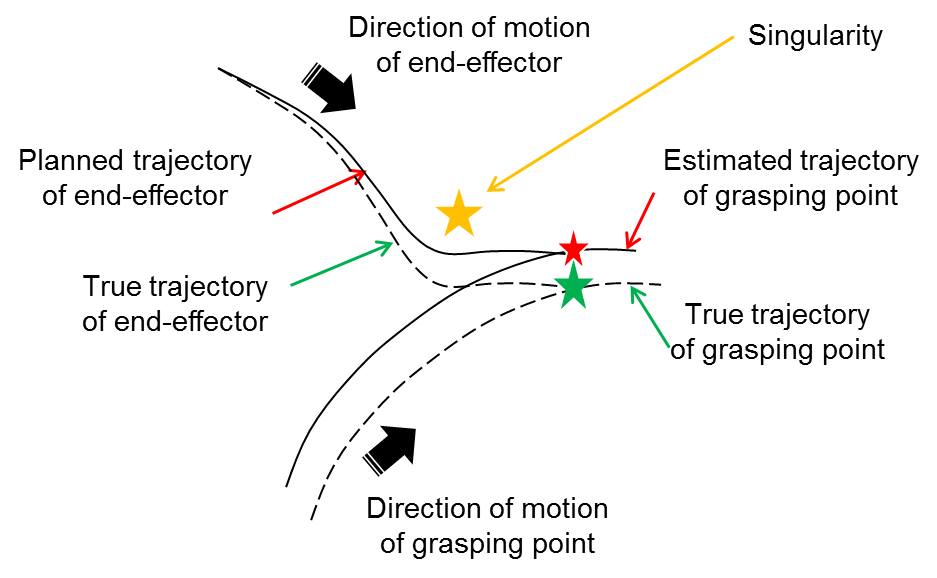
\includegraphics[angle=0,width=0.42\textwidth]{Motivation_Image.png}
\caption{The motion of the Target grasping point and of the robot end-effector are shwon for the model-based (solid line) and for the true (dotted line) cases.}
\label{fig:motivation}
%\vspace{-10pt}
\end{figure}
%
\subsection{Problem statement}
% 0.5 pp
%
In the grasping task of interest we assume that the Target has a known geometry, such that model-based computer vision pose estimation can be used. Its angular rate is limited here to 2 deg/s (due to hardware limitations, the limit for the stabilization phase is set to 1 deg/s). %to provide pose estimates between the Target body reference frame and the robot end-effector frame. 
The grasping point on the Target is predefined. %We assume that its motion may be predicted for motion planning purposes [isairas2005] %and is limited in the maximum angular rate modulous to 2 deg./s. (due to hardware limitations, the limit for the stabilization phase is 1 deg/s). %We also assume that the dynamic paratemers of the Target are given with some given level of uncertainty (note that these are identified for motion prediction purposes only to an arbitrary constant [isairas2010]).
%
The Chaser is not actuated (free-floating) and is initially in the same orbit as that of the Target with zero translational and angular velocities.
%space robot consists of a 7 DoF robot manipulator mounted on a free-floating base, the latter not having any GNC actuation active during the task execution. We assume here that the grasping point is in reach of the robot for the complete grasping task. As such, we assume that the Chaser station-keeping has placed the Chaser in the same orbit as that of the Target, in the -V-bar direction, see Fig. ???, with an accuracy of ?? cm, ?? deg., ?? cm/s and ?? deg/sec.. The chaser initially has zero momentum (for the general treatment of the case of non-zero initial momentum see [Ale]).

The grasping task itself is commonly divided into three phases [IROS13]: an approach phase, in which the robot end-effector is brought above the moving grasping point of the Target; a tracking phase, in which the end-effector follows the grasping point with the same velocity, while homing in onto it and closing the grasp; a stabilization phase, in which the relative velocity between the Chaser and the Target is brought to rest by a suitable control of the robot manipulator. 

A feasible trajectory to accomplish this task is provided by a motion planner, first described in [IROS13] and extended here. The motion planner relies on a prediction of the Target motion, which can be accomplished as described in [isairas2005][Aghili][Dobowsky?]. However, in order to complete the task, the tracking controller will initially need to deviate from the reference trajectory, given that the latter is model-based and will differ from the real-world conditions. This fact is shown pictorially in Fig.~\ref{fig:motivation}. Note that the gross motion of the motion planner is still maintained, in order to avoid motion constraints such as, for example, a singularity. 

Due to the deviation from the reference trajectory in the approach and tracking phases, the reference trajectory for the stabilization phase is adapted online, such that the deviation in joint space is recovered. This favours the fullfillment of joint position related constraints (collisions avoidance, singularity avoidance) throughout it. 
%
%It remains to be shown, as we do here, that the reference trajectory can be used by a tracking controller to accomplish the complete grasping task, to include the stabilization. The assumption is in fact that errors in the reference trajectory for the approach phase are sufficiently small. 
%
%If not, the reference trajectory for the stabilization phase may become unfeasible. In fact, while in the approach phase the visual servoing takes care of the necessary trajectory motification, in the stabilization phase, the robot joint controller returns to the reference trajectory, in order to ensure that joint position related constraints (collisions avoidance, singularity avoidance) are fullfilled throughout it. More wil be said about this in Section ???.
%
%In this way, by grossly tracking the reference trajectory the feasibility of the complete maneuver is guaranteed. As such, the end time of the stabilization phase need not be minimal, as suggested in [Aghili], since it is sufficient that the system remains in the vicinity of the planned trajectory, and may be chosen following a different cryterion. Minimum energy maneuvers can be considered as a viable alternative, since, as we will see, they are more robust to modelling errors and visual servo inaccuracies.
%
%Since we also want to be able to deal with a contingency case, for which an undesired impact between the robot and the Target may occur (CHECK need to demonstrate in experiments?), the feedback control method is based on impedance control. This allows to handle the case of an impact robustly, by suitably tuning the impedance []. Furthermore, the possibility of losing the Target after the impact is further greatly reduced by the visual servo.
%
%The aim of the experimental validation includes testing and analysis of the vision guidance (pose estimation), the robot planning, the robot controller, as well as taking imperfect attitude control and robot manipulator control into account. Differently to other works of this kind cited above, due to the macro-micro kinematic structure of our facility, we can include all these elements together in one test environment. Last but not least, the realistic nature of the uncertainty is enhanced in the experimental setup, by the latters's time discretization, time delays, kinematic modelling errors, etcetera. 
%
%Motivation for VS: uncertainty coming from motion prediction (+/- 10 cm in real system), LUT approximation (i.e. solution for desired point is not exact, but how much?), robot model uncertainties (<1 cm), robot controller positioning error (+/- 2 cm), GNC positioning error (+/- 5 cm), GNC velocity error (+/- ? cm/s - see DEOS), unmodelled disturbances (?) - need a scaling rationale: test sum of erros on 3m long robot to see what joint error is to be expected and scale error here accordingly, accounting fr nonlinearity, or validate tests in simulation just as much + look for trajectories for which this error is least visible in joint space!
%
%\section{Robot autonomy and on-orbit servicing}
%
%It is interesting to realize that, as mentioned in Section ??, two different control approaches are foreseable for the grasping task: the telepresence-based and the autonomy-based approaches. The dibate whether one can supersede the other is still open, since both have their benefits and flaws. The first can make use of the operator's intelligence, to include promptness in dealing with unexpected operational conditions and more robustness to adverse lighting conditions. At the same time, the benefit brought by a delayed force reflection (between 30ms and 600ms, for direct and Geo Relay links respectively) to an operator on ground, when executing the grasping of a tumbling Target, is still being investigated upon. Evidence of the difficulty for humans to generally perform this task is already provided in [Aghili's x2], although these used position-controlled robots with low controller sampling rates (check).
%
%On the other hand, autonomous systems are often favoured in industry-driven studies (see for example DEOS and eDeorbit) because of different reasons: the high bandwidth requirements of telepresence (DEOS); the fact that the round-trip-time needs to include the operator reaction time, typically taken to be one second, which in the case of a contingency during grasping may be decisive (eDeorbit); the communication window is limited in the case of a direct link, by the limited ground station coverage, as well as by the possibility of occlusion brought about by the same tumbling Target; communication through a geostationary relay satellite may pose hard challenges in the antenna pointing task, if the Chaser is in synchronized flight with the Target (eDeorbit); finally, the autonomous mode guarantees feasibility with respect to the non-intuitive stabilization task, which was not addressed in the telepresence approach to date.
%
%+ see arguments from Aghili in favour of autonomy.
%
\section{Methods}
%
In this Section we present the methods used to solve the grasping task, to include (CHECK) elements of the motion planning, the visual-servo-based tracking control used in the approach and the tracking phases and the joint-position-based tracking control used in the stabilization phase. The control system architecture is shown in Fig.~\ref{fig:blockdiagram}.

Define reference frames: inertia, chaser (?), end-effector, target, grasping point. Diagram needed?
%
\begin{figure*}
\centering  	\label{fig_1}
\psfrag{text_tr}[cc][cc][\FontFigM]{\textbf{Target tracking}}
\psfrag{text_st}[cc][cc][\FontFigM]{\textbf{Stabilization}}
\psfrag{text_vs}[cc][cc][\FontFigM]{Visual Servo}
\psfrag{text_pd}[cc][cc][\FontFigM]{\small{\begin{tabular}{@{}l@{}} Compliant\\Controller\\(PD+nullspace\end{tabular}}}
\psfrag{text_pl}[cc][cc][\FontFigM]{\small{\begin{tabular}{@{}l@{}} Plant\\(Chaser\\+manipulator\\dynamics\end{tabular}}}
\psfrag{text_mp}[cc][cc][\FontFigM]{{\begin{tabular}{@{}l@{}} Motion\\Synthesizer \end{tabular}}}
\psfrag{text_js}[cc][cc][\FontFigM]{\small{\begin{tabular}{@{}l@{}} Joint-space\\stabilization\\controller \end{tabular}}}
\psfrag{t1}[cc][cc][\FontFigM]{\small{\begin{tabular}{@{}l@{}} Camera\\Vision \end{tabular}}}
\psfrag{t2}[cc][cc][\FontFigM]{\small{\begin{tabular}{@{}l@{}} EKF\\Observer \end{tabular}}}
\psfrag{txt_k}[cc][cc][\FontFigM]{\small{\begin{tabular}{@{}l@{}} Kinematics\\(Base/manipulator) \end{tabular}}}
\psfrag{t4}[cc][cc][\FontFigM]{\tiny{$\begin{bmatrix}q(t_g)\\ \dot{q}(t_g)\end{bmatrix}$}}
\psfrag{EKF_out}[cc][cc][\FontFigM]{\tiny{$\hat{H}_{eg}$}}
\psfrag{cam}[cc][cc][\FontFigM]{\tiny{$H_{eg}$}}
\psfrag{ts}[cc][cc][\FontFigM]{\tiny{$10$ [Hz]}}
\psfrag{t_3}[cc][cc][\FontFigM]{\tiny{$\tau$}}
\psfrag{mp_car}[cc][cc][\FontFigM]{\tiny{$\begin{bmatrix}H_{eg,ref}\\ V_{eg,ref}\end{bmatrix}$}}
\psfrag{t_5}[cc][cc][\FontFigM]{\tiny{$\begin{Bmatrix}V_{e} & \dot{q} & H_{e} & q\end{Bmatrix}$}}
\psfrag{mp_joint}[cc][cc][\FontFigM]{\tiny{$\begin{bmatrix}q_{ref}\\ \dot{q}_{ref}\end{bmatrix}$}}
\psfrag{vs_out}[cc][cc][\FontFigM]{\tiny{$\begin{bmatrix}H_{e,des}\\ V_{e,des}\end{bmatrix}$}}
\psfrag{cc_out}[cc][cc][\FontFigM]{\tiny{$\begin{bmatrix}\tau_{cart}\\ \tau_{null}\end{bmatrix}$}}
\psfrag{int}[cc][cc][\FontFigM]{$\int$}
\psfrag{V_e}[cc][cc][\FontFigM]{\tiny{$V_e$}}
\psfrag{H_e}[cc][cc][\FontFigM]{\tiny{$H_e$}}
\psfrag{j}[cc][cc][\FontFigM]{\tiny{$\begin{bmatrix}q\\ \dot{q}\end{bmatrix}$}}
\psfrag{H_T}[cc][cc][\FontFigM]{\tiny{$H_t$}}
\centering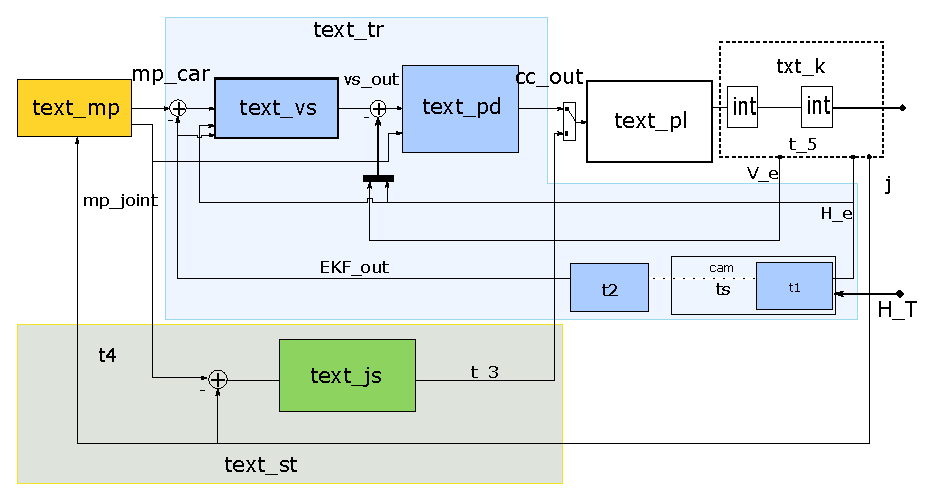
\includegraphics[angle=0,width=0.95\textwidth]{BlockDia1.eps}


\caption{Control system architecture with...}
\label{fig:blockdiagram}
\end{figure*}
%
%\begin{figure*}
%\centering\includegraphics[angle=0,width=0.95\textwidth]{./figures/Block_diagram_stabiliz}
%\caption{Control block diagram for the stabilization phase.}
%\label{fig:blockdiagram2}
%\end{figure*}
%
%\subsection{Control system architecture - 0,5 pp}
%
%A block diagram of the control systems for the approach and tracking phase and for the stabilization phase are shown in Fig.~\ref{fig:blockdiagram} and Fig.~\ref{fig:blockdiagram2} respectively. 
%
%\subsubsection{Plant}
%The plant refers to the free-floating robot, consisting of a free-floating satellite base and a 7 DoF robot manipulator. The only actuators present are those of the robot joints, since the base is assumed to be non-actuated. The sensors include the position and torque sensors of the robot joints and a stereo-camera at the robot end-effector. The satellite states are assumed to be ideal (check).
%
%Define reference frames. inertia, body, end-effector, other.
%
%\subsubsection{Target}
%This block represents the simulation of the Target motion, including that of the predefined grasping point on it.
%
%\subsubsection{Motion synthesizer}
%The motion synthesizer receives the reference trajectory from the motion planner and interpolates the desired Cartesian pose and robot configuration in time. Note that this function runs on-board of the Chaser spacecraft, whereas the reference trajectory is generated on ground before the task is executed.
%
%\subsubsection{Robot controller and forward kinematics}
%This is the inner loop of the robot controller, which runs at a sampling time of 1KHz. It containts two elements to control both the Cartesian pose and the joint configuration in null space. The forward kinematics provides the current Cartesian pose of the robot end-effector through a forward kinematics computation. The robot controller then, based on the chosen control strategy (see Section ??), determines the control torques to be applied to the robot. The satellite states are assumed to be ideal (check).
%
%\subsubsection{Camera-based motion estimation}
%This block represents the computer vision algorithm which runs onboard at a slower sampling rate of 10Hz and which provides the current relative pose between the robot end-effector and the Target grasping point (check). 
%
%The connections between these blocks constitute the visual servo and will be addressed in Section ?? in detail.
%
\subsection{Motion planning and motion synthesizer}
% - 1 pp
%
The motion planning method adopted in this work is described in some detail in [$Lampariello_IROS2013$] - check. We provide here extensions of it, to account for requirements stemming specifically from the visual servo and the joint tracking control and to improve the quality of the solutions presented in [$Lampariello_IROS2013$] with regards to the stabilization phase. Check - need to describe method and solutions in some more detail.

\subsubsection{Motion planning constraints during approach phase}
%

Add: camera-filed of view (constraint on beta check) and end-effector velocity (partially removed velocity jump; define pixel velocity and its constraint); underline outputs: end-effector pose AND robot joint positions PLUS explanation of effect of disturbances (plot as in notepad?); cost function?; look for singularities

In order to feed the motion planner solutions described in [$Lampariello_IROS2013$] to the robot controller some adaptations were necessary. The most important were related to motion constraints on the camera-field of view direction, such that the Target remains in view throughout the complete approach phase, as well as on the end-effector velocity (check), such that the pose estimator can perform the tracking in a stable manner (check - expand and/or reformulate):

Equations of e-e direction constraint - analyze again and maybe add new method with cone? since straightforward method has local minima.

The velocity jump between the end of the approach phase and the beginning of the tracking phase was removed, for better performance (check). The latter was also greatly improved by providing the trajectory in form of the relative pose with respect to the Target, ??, but also of the velocity and acceleration (check, also if other). Check for other constraints.

Underline importance of singularities as a motion constraint, since it is not known where they are (esp. in function of load mass, but check Cusumano's) and fact that we need to track grasping point. Methods which use redundancy do not guarantee at all times that grasping point can be tracked at all times (CHECK), since might ahveto deviate path or bring velocity to zero. Furthermore, we don't know if then restofmotion is feasible, since have completely new robot configuration.

\subsubsection{Motion planning for the stabilization phase}

Add: online recomputation (see equations in algorithm); cost function LWR mechanical energy plus reason; global search (shows that there are local minima, details of search); other (see notes)

"In this way, by grossly tracking the reference trajectory the feasibility of the complete maneuver is guaranteed. As such, the end time of the stabilization phase need not be minimal, as suggested in [Aghili], since it is sufficient that the system remains in the vicinity of the planned trajectory, and may be chosen following a different cryterion. Minimum energy maneuvers can be considered as a viable alternative, since, as we will see, they are more robust to modelling errors and visual servo inaccuracies."

Stress that it is a rigidization, not a stabilization/detumbling), considering compound, best robot motion for chaser to absorb and share target's momentum, total momentum remains constant.

The optimization problem for the stabilization phase was treated in a similar way as the approach phase. The joint states were parameterized with B-slines and provided the initial conditions in position, velocity and acceleration (check) resulting at the end of the tracking phase. The final conditions on the joint states were only expressed for the joint velocities and accelerations, leaving the joint positions open for the optimizer to be determined, in function of the assigned cost function. Note that this point solves an open issue when only implenting a dissipating control law, to stabilize the compound. In fact, doing so firstly does not give any bound on the final position reached at the end of the motion and as such no guarantee that collisions are avoided. Secondly, due to noise in the system, a purely dissipative control law results in a continuously drifting system (check with Marco and add results later?). The number of parameters was increased, for better convergence performace. 

Of notice here is also to realise that the choice of parameterizing the robot joints was favoured with respect to that of parameterizing the end-effector trajectory. This is firstly because the robot control needs joint position commands, which in our case are given directly from the solution, without having to revert to an inverse kinematics function, to great advantage of the motion synthesizer (see Section ??). The use of an inverse kinematics function is also generally not advisable for the case that a singularity is met. In this case, the inverse of the Jacobian is undefined. However, we note that singulatities also provide numerical problems in the presented formulation, due to the fact that even in their vicinity, the joint velocities increase noticeably. The integration of the equations of motion of a free-floating system is very sensitive to large velocities, leading the necessity of an excessively small integrator step size. Check - show example in results?

Results: tau for $m_servicer = inf$ is a lot higher than for $m_servicer = 500$ - show solution and joint taus for both cases? Plus say that total momentum remains constant. Following target trajectory and slowing it down does not take account of chaser inertia. Providing a MBS solution vs Aghili's single rigid body solution. Show joint curves with zero jerk, for minimizing solar pannel excitation (min time is not ideal for this).

%\subsubsection{Motion planning cost function}

With regars to the cost function, we chose here to minimize the mechanical energy. We propose it as alternative to minimizing the end time given that we track the solution in joint position and as such guarantee the collision avoidance that could arise from any residual relative drif velocity between the two spacecrafts. Although minimizing the mechanical energy requires defining a final time, since the solution would otherwise push the end time to infinity, an arbitrary sensible value can be chosen by the user, after inspection of the first solutions. It is important to stress that the goal of the motion planner is first to provide a feasible solution. The optimality is then used to make the solutions more robust to the uncertainties. Finally, due to the highly nonlinear nature of the problem (check), a global search is performed, in order to find a (close to) global minimum for a given query. Although we do not address the task of generating a look-up table here, for any tumbling state of interest, we revert the reader to [IROSD2013] for further details on this point.

21/12/2017: the chosen cost function for the rigidization is the integral of the product $tau*qd$. This is best to option to reduce the effort of the LBR! Only drwaback is that is does not look nice, i.e. the target rotates toward the chaser (did a global search and could not find any better solutions). The integral of the product $F_e*v_e$ could be an interesting alternative (given that it implies a solution where the target slows down along its path, without rotating toward the chaser) to minimize the risk of collision, although we can deal with that.


End of current version


Explain motion synthesizer - give details of on-line B-spline with on-line modification function of new robot joint states + Phillip, Marco + see how this can work on board for all required outputs to controller! Then explain how Cartesian trajectory could be modified with motion prediction during approach and how resulting cartesian reference trajectory could be perfectly updated to real motion (relative to the base body). But must chose to give preference to joint position error (which neglects target trajectory change, otherwise don't know where will end up) and possible collision avoidance or to Cartesian error and possible end-effector and joint torque error (show how this can grow, for a given trajectory error!). As such minimizing energy gives a smooth solution and as such a more robust solution to prediction errors, since far from the motion boundaries and not on the edge of them (optimal handling of uncertainties on the off-line generated motion plannign solutions). Favoured here avoiding singularities. Furthermore, say that for LBR on OOS-SIM 5 cm error are a lot, but for 3/4 m long arm not. 

Say that: The presented method needs to be able to meet strict guarantees on the solution (such as the upper bound on the computation time), for the safety-critical application at hand (software ceritifcation processes also need to be considered). As such, all computations involving optimization algorithms have to be performed off-line on ground. 


Maybe put all these choices in the results discussion section.


0. motion planning (Roberto):
	v. say that opt. params for Chaser position are very important for good convergence properties - but add params in approach to improve convergence - to do!
	vi. say about minimizing joint motion or joint motion in null-space for approach phase - see use of nullspace term in invkin (see dkin2!!!) - to reduce effect of friction in NS dynamics of real robot - talk to Christian.
	vii. say that for LBR on OOS-SIM 5 cm error are a lot, but for 3/4 m long arm not.
	viii. compare min energy solution to solution from $F_e=K_d * Deltax_dot$ (must implement), for different Chaser/Target mass ratios
	ix. do global search for min energy or command given $v_e, omega_e$ to inv-kin to see solution
	x. add $q_ddot$($tf_approach$) as parameters to minimize tau($0_tracking$)
	xi. compare joint space to cartesian space stabilization solution approaches
	x. the problem of extracting the optimal solution from the LUT is not addressed in any more detail here (see IROS 2013)

In pp method?
In the proposed method, a motion planner provides a reference trajectory to execute the task described above, details of which can be found in [IROS2013]. Of notice it the fact that the method in [IROS2013] is meant to firstly guarantee the feasibility of the task with respect to all motion constraints, described in Section??. This differes from any of the approaches described in Section???, since there many important constraints are either not treated exhaustively (e.g., joint position and velocity, the latter in view of dynamic singularities, the position of which for a ff 3D system with n dof and with load X on e-e cannot be predefined to date), implying that the explicit effect of a disturbance or uncertainty on the future evolution of the system is not taken into account, or only added in the cost function as a weighting term (e.g., line-of-sight of end-effector cameras, for which the useful Target features may be lost, with obviously negative consequences), thus not guaranteeing their fullfillment. Here instead, the method based on nonlinear optimization, guarantees the fullfillment of the constraints for the reference trajectory (at the chosen via points, of arbitrary number, sufficient for the task). Due to the highly non-linear nature of the problem, the presented method also provides a (near to) global optimimum, for a very wide range of cost functions, for example,  minimized for improvement of the robustness of the control method, to model uncertainties and sensor errors, by performing a global search for a given task. The method finally allows to represent the system in question in its full free-floating dynamic behaviour, without the need to reduce the Chaser dynamics to those of a fixed-based robot, for ease of resolution of the related optimal control problem. We will see in Section ??? that the stabilization task is in fact a momentum transfer problem, rather than a detumbling (or passivation?) problem, with useful consequences on the resulting solutions found. The tumbling of the compound after the stabilization is by no means an issue, when realizing that the minimization of the attitude has been solved with simple technological solutions, such as omnidirectional antennas and gymbal joints [DEOS]. The impelling need for robot autonomy for the grasping task was also made evident in [eDeorbit], underlining the need for full autonomy, for which a communication link in the critical grasping phase is not foreseen.
+ In the same Figure, the necessity for a motion planner is underlined by showing how this deviates around a robot singularity, rather than going right through it, as a simple regulation controller would do.
+ make clear statements about singularities: although inv kin methods can avoid them, we can't tell if the motion after them is then feasible anymore, given non-holonomic nature of Chaser dynamics + if cannot avoid them right during tracking, we have a problem + cannot represent them yet.
+ The uncertainties are quantified and analysed here to some extent, to validate the truthfullness of the assumption. 
+ This last point has required making a decision between prioritizing position related to force related constraints. The internal forces required for the adjustment of the trajectory in the stabilization phase are function of the tracking error in the approach phase, and as such unknown. The alternative would be to recompute the stabilization trajectory online in cartesian space and tranfer the unknown onto the final position reached by the robot... 
+ The feasibility (region) is provided by the motion planner, not by the user [Aghili's ball]. 
	
%
\subsection{Visual Servo for Approach and Tracking Phases - 1 pp}
%

% Hrishik
% Describe rational and method (equations) of visual servo
% Describe KF method, refer to existing literature (ASTRA?)

% Roberto
% Describe LWR impedance controller
% Describe null-space controller

1. Control Visual Servo Approach (Hrishik, Roberto)
        -i. describe how to command the planned trajectory to the visual servo (optimization offline on ground, what is done on-line on board?), such that it is grossely followed, both in Cartesian and in joint space, but at the same time corrected by the feedback controller, to account for modelling errors and other uncertainties.
	0. The visual servo is described in detail, to include tuning of an inner-loop impedance controller with an outer-loop visual servo, in the approach and tracking phase.
	i. updated DEOS block diagram (position and impedance control), feedforward term, other
	ii. inputs from path planner - e-e trajectory, configuration trajectory for null space, other
	iii. theory for tracking of relative motion
	iv. theory for tracking of null-space -ask Christian/Alin
	v. visual servo (computer vision, visual servoing)
	vi. robot control method for ff robot (Jg) and tracking control; what is maximum allowed impedance of LWR?
	vii. use of KF with preidentified model parameters, for CV failure (e.g., due to occlusions)
	viii. The satellite states are assumed to be ideal - check which are needed: $r0, v0, ori_0, omega_0$, sampling time (3 Hz, 1 kHz), other
	
\subsubsection{Computer Vision for Approach and Tracking Phases}

% Nassir

% describe CV method, refer to existing references
% provide analysis to explain why CV fails, with reference to experiemental data (image sequences)
The visual pose estimation is based on work of~\cite{Drummond2002} which relies on a known object geometry. The algorithm consisits of sampling model contours and edge detection, followed by a local optimization of the 3D rigd-body transform. The re-projection error is then minmized between visible model contour and image edges using Levenberg-Marquardt algorithm.
 %Related to this model matching approach is moving edges method~\cite{Comport2004} which differs from the former in contour samply strategy. The latter samples model contours in 2D, after projecting model lines on the image. These two approaches have their own advatnages and disadvantages which have been explored in~\cite{Comport2005}. While both approaches show similar performance, the former is easier to implement as it presents a direct and accurate formulation for minimizing the reprojection error from %3D to 2D~\cite{Oumer2015}. 
The complex motion trajectory (tumbling and an abrupt change of angular velocity) of the target poses difficulty in visual tracking. In order to address this problem, a motion prediction scheme based on the extended kalman filter is integrated into the local optimization. The prediction relies on a simple kinematic motion model assuming constant frame to frame motion. Under this assumption, the visual tracker is able to cope with relatively higher image motion between two camera frames. Moreover, the short-term prediction scheme helps the visual tracker reduce the search space in order not to trap in potential local optima during minimization of the cost function. The qualitative tracking results are illustrated in Fig.~\ref{fig:TrackingImages}, with an examplar tracked images during approach and tracking phases. Those in red indicate the projection of model contours on to the image edges at the estimated pose. The axes of the coordinate frame of grasping point are indicated in red, green and blue. The overlap of the model contours and image edges shows the successful tracking and pose estimation.

%\begin{figure}
%\centering
%\begin{subfigure}
%	\includegraphics[angle=0,width=0.95\textwidth]{./figures/frame0786_result_cam0}
%	\caption{approach}
%\end{subfigure}
%\begin{subfigure}
%	\includegraphics[angle=0,width=0.95\textwidth]{./figures/frame0849_result_cam0}
%	\caption{Tracking}
%\end{subfigure}
%\begin{subfigure}
%	\includegraphics[angle=0,width=0.95\textwidth]{./figures/frame0922_result_cam0}
%	\caption{Tracking}
%\end{subfigure}
%\begin{subfigure}
%	\includegraphics[angle=0,width=0.95\textwidth]{./figures/frame0954_result_cam0}
%	\caption{Tracking}
%\end{subfigure}
%\label{fig:TrackingImages}
%\caption{Exemplar images during visual tracking for approach and tracking phase. The overlay of the model contours and image edges shows the successful tracking and pose estimation. The %target features reduce significantly as the manipulator approaches close to grasping. The axes of the coordinate frame of grasping point is indicated in red, green and blue }
%\end{figure}


%
\begin{figure*}
\centering\includegraphics[angle=0,width=0.24\textwidth]{frame0786_result_cam0}
\centering\includegraphics[angle=0,width=0.24\textwidth]{frame0849_result_cam0}
\centering\includegraphics[angle=0,width=0.24\textwidth]{frame0922_result_cam0}
\centering\includegraphics[angle=0,width=0.24\textwidth]{frame0954_result_cam0}
\caption{Exemplar images during visual tracking for approach and tracking phase. The overlay of the model contours and image edges shows the successful tracking and pose estimation. The axes of the coordinate frame of grasping point is indicated in red, green and blue. The target features reduce significantly at very close range because of gripper occlusion (black in the image) and camera field of view.}
\label{fig:TrackingImages}
\end{figure*}


%There exist, however a few cases where the visual tracking was not able to provide the required pose accuracy for the visual servoing. For example, the inherent vision-based %pose estimation problem assocociated to in-plane motion where lateral rotation estimation error is large, particularly when a partial surface of the target with planar geometry is momentarily visible in non perspective view. Moreover, the outliers due to occlusion and limited field of view poses tracking failure particularly at very close range, as shown in Fig.~\ref{fig:GraspingImages}. Fortunately, at this range the gripper is a few millimeters from the grasping point, hence the implemented motion predictor supports final grasping phase.

%\begin{figure}
%\centering
%\begin{subfigure}
%	\includegraphics[angle=0,width=0.95\textwidth]{./figures/frame0954_result_cam0}
%	\caption{approach}
%\end{subfigure}
%\begin{subfigure}
%	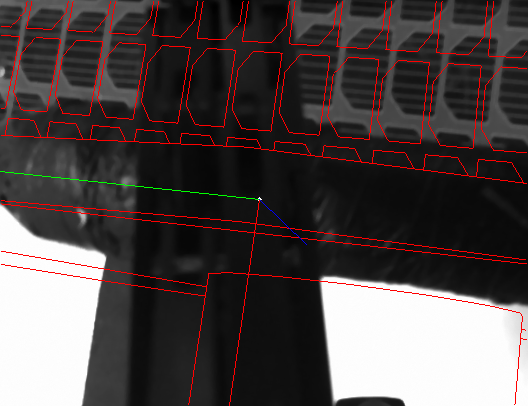
\includegraphics[angle=0,width=0.95\textwidth]{./figures/frame0955_result_cam0}
%	\caption{Tracking}
%\end{subfigure}
%\begin{subfigure}
%	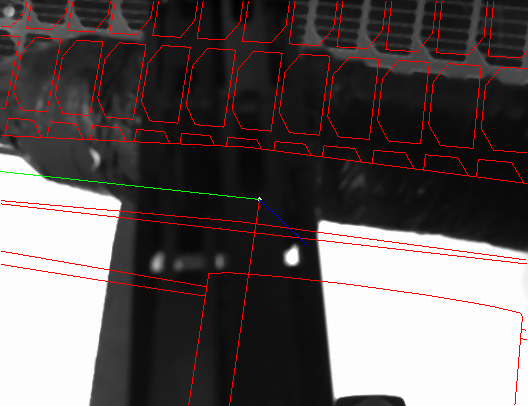
\includegraphics[angle=0,width=0.95\textwidth]{./figures/frame0956_result_cam0}
%	\caption{Tracking}
%\end{subfigure}
%\label{fig:GraspingImages}
%\caption{Failure cases of the visual tracking. At very close range, the visible target features are not sifficient for pose estimation because of occlusion (black in the images) and  %reduced field of view}
%\end{figure}

%\begin{figure*}
%\centering\includegraphics[angle=0,width=0.24\textwidth]{./figures/frame0954_result_cam0}
%\centering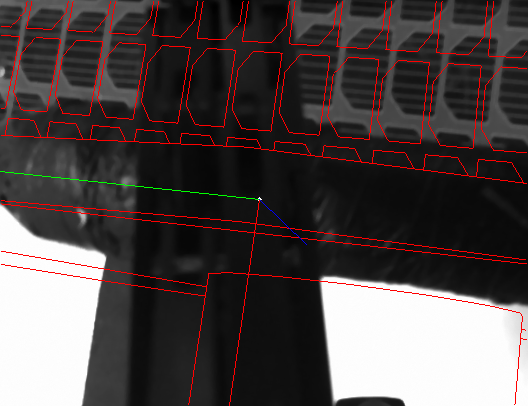
\includegraphics[angle=0,width=0.24\textwidth]{./figures/frame0955_result_cam0}
%\centering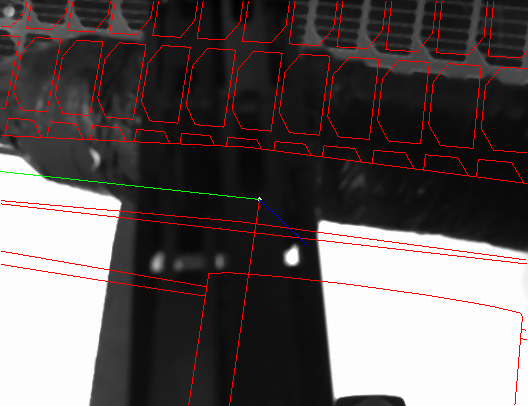
\includegraphics[angle=0,width=0.24\textwidth]{./figures/frame0956_result_cam0}
%\caption{Failure cases of the visual tracking. At very close range, the visible target features are not sifficient for pose estimation because of occlusion (black in the images) and  reduced field of view.}
%\label{fig:GraspingImages}
%\end{figure*}

% ---- You may menstion this in future work section-----
%In the future, the performance of the visual tracking will be improved, addressing problems related to in-plane motion, local minima and large image pixel velocity by integrating dynamic motion model of the coupled satellite-manipulator system for long-term prediction. Moreover, the visual tracking will be validated in a representative space environment with proper lighting conidtion as in~\cite{OumerPhdThesis}.

%	i. The visual servo also includes a pose estimation algorithm, which relies on a predefined simplifies model of the Target - show image with simplified model of the target

%
\subsection{Joint Tracking Control for Stabilization Phase - 0,5 pp}
%

% Roberto or Marco
% Describe tracking controller
% 

2. Control Stabilization (Marco, Roberto)
	i. updated DEOS block diagram (position and impedance control), feedforward term, other
	ii. inputs from path planner
	iii. robot control method for ff robot and tracking control
	iv. add e-e force contraints, e.g. to avoid slipping after grasp
	v. say that now we can add a proportional term, since we know where to bring the system - not just a damping term.
	vi. Remind that tracking guarantees feasibility. As such minimum time is useless and relative drift is compensated for by robot.
	vii. cite Satoko/Lampariello paper for impedance controller as comparison.
%
\section{Experimental facility - 0.5 pp}

% Roberto
	
	i. introduce falicity
	ii. describe extensions: target motion, post-grasping tumbling motion
	iii. 4N/1Nm (CHECK) deadband in Target FTS - removed after grasping
	iv. End-effector pads to avoid slipage (?)

%
\section{Results - 1 pp}

Simulation (Roberto):
	i. analysis of motion planning solution - global search results, cost functions, motion constraints; add a post-processing of the data in log.txt to show the evolution of the optimizer iterations to the solution
	ii. comparison to Aghili's approach and solutions, analyse mom. + k.e. before and after
	iii. analyse robustness of solutions to uncertainty
	iv. provide numbers on field-of-view constraints and graph that meets that
	v. show exemple with singularity
	vi. comparison simulation of mission scenario with experimental facility (till contact)

Cost functions: 
	- target k.e.: given nice target motion
	- robot mech. energy: is much better in comparison to target k.e. in terms of optimal value, but target motion is out-of-plane
Compare solutions:
	- see notes at the end of readme.txt: plot e-e vel and e-e pos.
	- plot also $q_ddot$ to show smoothness from end of tracking to beginning of stabilization
	- plot $F_e$ and $tau_e$ (derive from computation of e-e acceleration? Or from solution of $tau=J_T Fe$?) and cf to $v_e$ and $omega_e$. 	Is $tau_e$ parallel to $omega_e$? Should be and see Aghili's analytical solutions as comparison.
Optimizer settings:
	- compare mine with Joos's
	- compare vels and acc in transition from tracking to stabilization: use vel in $DATA/Output_control_invkin_base_joints_vels.dat$ - 			plot(out1(:,1), out1(:,8:14)), but need the values half way along the data, since invkin integrates for twice the length of tracking 			phase, so do n=size(out1), out1(n/2,8:14)  - for tracking phase and $DATA/Results_joints_vel_stabil.dat$ - for the stabilization. Show 			plot: 
	
	figure(1); plot(out1(1:142,1), out1(1:142,8:14))
	hold on; plot(out2(:,1)+out1(142,1), out2(:,2:8))


VS, KF, Controller (Hrishik, Marco):
	i. tuning details
	ii. performance details
	iii. Assumptions: the satellite states are assumed to be ideal or rather in the operational window defined above - check which are needed: $r0, v0, ori_0, omega_0$, sampling time (3 Hz, 1 kHz), other. See how to treat this issue in reality (discussion with Alessandro)


Experiments (Roberto, Hrishik, Marco):
	i. experimental facility description - add changes applied for Institutsueberpruefung: post-capture motion as a momentum conservation task, 3D target motion, other
	ii. examples with different tumbling target states - success of tracking and of satisfying motion constraints, cost function in experiments vs in simulation
	iii. null-space motion tracking
	iv. end-effector force slip limit satisfaction
	iii. comparison to regulation approach? Show that less robust and can become faulty due to motion constraints
	iv. solution for CV frame loss, i.e. performance of KF on-line
	v. performance analysis with modelling/prediction error
	vi. show open-loop motion with impact on target
	vii. show singularity with N45 (or N30) and inertia servicer divided by 10 - perhaps seen on OOS-SIM

%
\begin{figure}[t!]
\psfrag{y1}[cc][cc][\FontFigB]{$||\Delta r_c||^2$}
\psfrag{y2}[cc][cc][\FontFigB]{$||\Delta r_c||^2$}
\psfrag{leg1}[cc][cc][\FontFigS]{$EKF$}
\psfrag{leg2}[cc][cc][\FontFigS]{$Vision$}
\psfrag{x}[cc][cc][\FontFigS]{$EKF$}
\psfrag{y}[cc][cc][\FontFigS]{$Vision$}
\psfrag{t}[cc][cc][\FontFigB]{$t$[sec]}
\psfrag{ekf}[cc][cc][\FontFigS]{$EKF$}
\psfrag{vision}[cc][cc][\FontFigS]{$Vision$}
\centering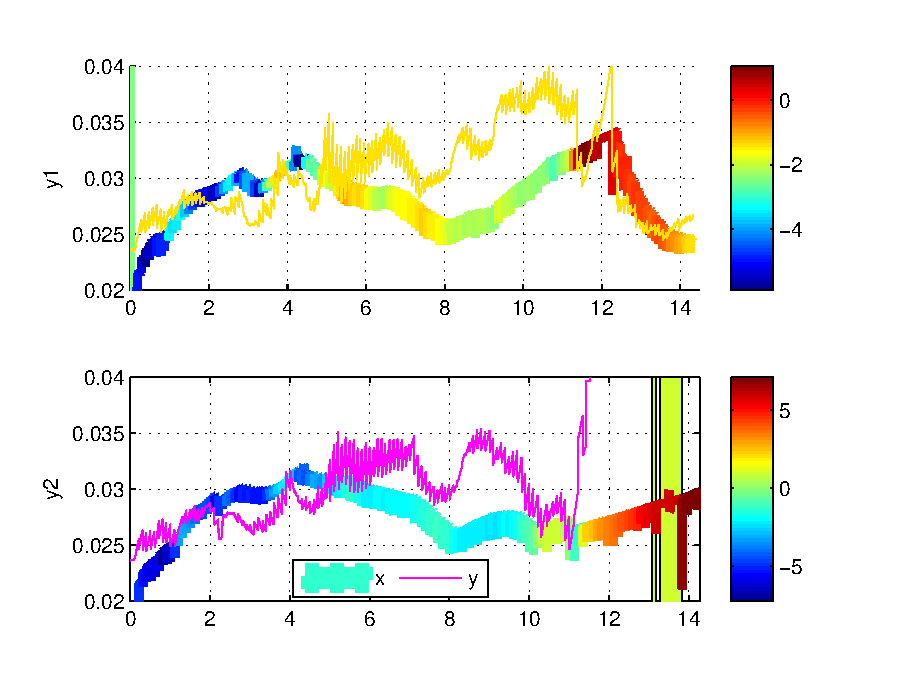
\includegraphics[angle=0,width=0.47\textwidth]{fig_norm_errors.eps}
%\resizebox{0.48\textwidth}{!}{\fontsize{200}{200}\selectfont{\input{motiv.pdf_tex}}}
\caption{Comparison of direct-Vision measurements with EKF, based on the norm, $||\Delta r_c^2||$. As $||r_c|| \rightarrow 0$, the statistical measure of fitness, $\chi^2 \rightarrow \infty $ eventually leading to pose estimation failures due to degenerate observability}
\label{fig:res_1}
%\vspace{-10pt}
\end{figure}
\begin{figure}[t!]
\psfrag{om}[cc][cc][\FontFigB]{$\omega$}
\psfrag{omhat}[cc][cc][\FontFigB]{$\hat{\omega}$}
\psfrag{true}[cc][cc][\FontFigB]{$\omega$}
\psfrag{t2}[cc][cc][\FontFigB]{$t$[sec]}
\psfrag{t1}[cc][cc][\FontFigB]{$t$[sec]}
\psfrag{qua}[cc][cc][\FontFigB]{$\mu$}
\psfrag{qhat}[cc][cc][\FontFigB]{$\hat{\mu_{EKF}}$}
\psfrag{vision}[cc][cc][\FontFigB]{$\mu_V$}
\centering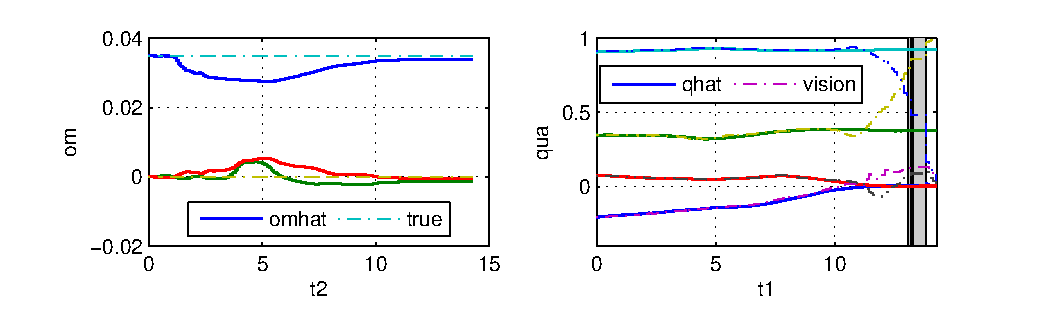
\includegraphics[angle=0,width=0.47\textwidth]{states_EKF.eps}
%\resizebox{0.48\textwidth}{!}{\fontsize{200}{200}\selectfont{\input{motiv.pdf_tex}}}
\caption{a) Target state estimation ($\omega$) in EKF for tracking control. b) Divergence of Computer vision's orientation estimate towards end of maneuver}
\label{fig:res_1}
%\vspace{-10pt}
\end{figure}
\section{Conclusion - 0,25 pp}

- Shown feasibility of method (pp, VT for approach with CV and KF, tracking, grasp, stabilization), with experimental results on OOS-SIM.

- rivedi tutti commenti in Aghili papers!

- describe complete story (isairas 2005, pp iros2013 and this), where here we focus on the third part. We here make the motion planning (of the type in IROS2013) useful for control purposes, through the use of tracking control.

- since pp without feedback tracking control is no use for control purposes, we show here how the pp in [IROS2013] can be used exactly for this goal.

- See Balandat's statement (see above) + one on LUT idea. Therefore, we strongly believe that use of offline generated solutions retrieved on-line is the future, especially for complex tasks like grasping and stabilization in the presence of constraints (communication, other).

- still to do is validation with orbital lighting conditions.

- pp + VT for grasping is also new (said already). The stabilization task with a reference trajectory is new, with respect to the methods existing in the literature. 

- future work: include realistic illumination conditions, method to provide ref traj in useful time for complete taskspace.

- Said motivation for pp in Berlin talk, specific DEOS TN?

"Since we also want to be able to deal with a contingency case, for which an undesired impact between the robot and the Target may occur (CHECK need to demonstrate in experiments?), the feedback control method is based on impedance control. This allows to handle the case of an impact robustly, by suitably tuning the impedance []. Furthermore, the possibility of losing the Target after the impact is further greatly reduced by the visual servo."


%
\section{Videos}
1. simulation - bernhard
2. facility

%
%\section{Biblio} - 0,75 pp

@proceedings{Drummond2002,
Author = {T. Drummond and R. Cipolla},
title=  {Real-time visual tracking of complex structures},
booktitle= {IEEE Trans. Pattern Analalysis and Machince Intelligence},
pages = {932--946},
year = {2002}
}

@proceedings{Comport2004,
Author ={ A.I. Comport, E. Marchand, F. Chaumette},
title=  {Robust model-based tracking for robot vision},
booktitle= {Proceedings of the IEEE/RSJ International Conference on Intelligent Robots and Systems},
volume ={1},
pages = {692--697},
year = {2004}
}


@proceedings{Comport2005,
Author = {A.I. Comport, D. Kragic, É. Marchand, F. Chaumette},
title=  {Robust real-time visual tracking: comparison, theoretical analysis and performance evaluation},
booktitle={Proceedings of the IEEE International Conference on Robotics and Automation},
volume = {1},
pages = {2841–-2846},
year = {2005}
}

@article{Oumer2015,
title = {Vision-based localization for on-orbit servicing of a partially cooperative satellite},
author = {Nassir W. Oumer and Giorgio Panin and Quirin Mülbauer and Anastasia Tseneklidou},
journal = {Acta Astronautica},
volume = {117},
pages = {19--37},
year = {2015}
}

@phdthesis{OumerPhdThesis,
author = {Nassir W. Oumer}, 
title = {Visual Tracking and Motion Estimation for an On-orbit Servicing of a Satellite},
booktitle={Phd Thesis},
Address = {University of Osnabrück},
year = {2016}
}
